\documentclass{article}

\usepackage[english]{babel}

\usepackage{graphicx}

\usepackage{tabulary}

\usepackage{tabularx}

\usepackage{fixltx2e}

\usepackage[utf8]{inputenc}

\usepackage[dvipsnames]{xcolor}

\usepackage{tikz}

\usepackage{mwe}

\usepackage{xcolor}

%\textsubscript{this}

\usepackage{lastpage}

\usepackage[utf8]{inputenc}

\usepackage{ifthen}

\usepackage{amsmath}

\usepackage{fancyhdr}

\usepackage[document]{ragged2e}

\usepackage[margin=1in,top=1.2in,headheight=57pt,headsep=0.1in]{geometry}

\usepackage{fancyhdr}

\everymath{\displaystyle}

\usetikzlibrary{calc}

\usetikzlibrary{shapes.multipart, shapes.geometric, arrows}

\usetikzlibrary{calc, decorations.markings}

\usetikzlibrary{arrows.meta}

\usetikzlibrary{shapes,snakes}

\usetikzlibrary{quotes,angles, positioning}

\linespread{2}%controls the spacing between lines. Bigger fractions means crowded lines%

%\pagestyle{fancy}

%\usepackage[margin=1 in, top=1in, includefoot]{geometry}

%\everymath{\displaystyle}

\linespread{2}%controls the spacing between lines. Bigger fractions means crowded lines%

%\pagestyle{fancy}

\pagestyle{fancy}

\setlength{\headheight}{56.2pt}

\colorlet{Mycolor1}{green!10!orange!90!}

\chead{\ifthenelse{\value{page}=1}{\textbf \textbf Digestion Math Problems}}

\rhead{\ifthenelse{\value{page}=1}{Shabbir Basrai}{Shabbir Basrai}}

\cfoot{}

\lfoot{Page \thepage\ of \pageref{LastPage}}

\rfoot{Digestion Math Problems}

\renewcommand{\headrulewidth}{2pt}

\renewcommand{\footrulewidth}{1pt}

 

\makeatletter



 

%Defining colour with different models.

\definecolor{mypink1}{rgb}{0.858, 0.188, 0.478}

\definecolor{mypink2}{RGB}{219, 48, 122}

\definecolor{mypink3}{cmyk}{0, 0.7808, 0.4429, 0.1412}

\definecolor{mygray}{gray}{0.6}

\colorlet{LightRubineRed}{RubineRed!70!}

\colorlet{Mycolor1}{green!10!orange!90!}

\definecolor{Mycolor2}{HTML}{00F9DE}

 

%New command used in the table with all available colour names

\newcommand{\thiscolor}[1]{\texttt{#1} \hfill \fcolorbox{black}{#1}{\hspace{2mm}}}

 

%This changes the row separation in the table

\renewcommand{\arraystretch}{1.5}

\begin{document}

%This document present several examples on how to use the \texttt{color} package to change the colour of elements in \LaTeX.

 

\begin{itemize}

\item \textcolor{Mycolor1}{First item}

\item \textcolor{Mycolor2}{Second item}

\end{itemize}

 

%\noindent

{\color{LightRubineRed} \rule{\linewidth}{1mm} }

 

%\noindent

{\color{RubineRed} \rule{\linewidth}{1mm} }

 

 

Not only blocks, such as environments, can be set to a determined colour, but some \textcolor{red}{special words} too. You can even use your own user-defined colours. Below the same colour with different models:

 

\begin{enumerate}

\item \textcolor{mypink1}{Pink with rgb}

\item \textcolor{mypink2}{Pink with RGB}

\item \textcolor{mypink3}{Pink with cmyk}

\item \textcolor{mygray}{Gray with gray}

\end{enumerate}

 

%The background colour of some text can also be \textcolor{red}{easily} set. For instance, you can change to orange the background of \colorbox{BurntOrange}{this text} and then continue typing.

 

%\clearpage

 

%\begin{center}



%\end{center}%

 

\begin{tikzpicture}[scale=5]

\draw (.1,1.6) .. controls (.6,1.6) and (1.5,1) .. (2,1);

\draw (.1,1) .. controls (.6,1) and (1.5,.4) .. (2,.4);

\draw[dashed] (1,0) -- (1,2);

\end{tikzpicture}

 

\begin{tikzpicture}[scale=5]

\draw (0.1,0) .. controls (.6,1.6) and (1.5,1) .. (2,1);

\draw (0.1,1) .. controls (.6,1.6) and (1.5,1) .. (2,1);

\draw (0.1,2) .. controls (.6,1.6) and (1.5,1) .. (2,1);

\draw (0.1,0) .. controls (.6,1.6) and (1.5,1) .. (2,1);

\end{tikzpicture}

 

\begin{tikzpicture}[baseline=(current bounding box.north)]

 

% A clipped circle is drawn

\begin{scope}

    \clip (-1.5,0) rectangle (1.5,1.5);

    \draw (0,0) circle(1.5);

    \draw (-1.5,0) -- (1.5,0);

\end{scope}

%%

%%%Labels for the vertices are typeset.

%\node[below left= 1mm of {(-1.5,0)}] {$A$};

%\node[below right= 1mm of {(1.5,0)}] {$B$};

%\node[above right= 1mm of {(60:1.5)}] {$C$};

%\node[above left= 1mm of {(120:1.5)}] {$D$};

\end{tikzpicture}

 

 

 

 

 

\begin{tikzpicture} %[scale=3]

    \draw (0,0) node[below]{$O$} circle (2);

    \coordinate (A) at (120:2);

    \coordinate (B) at (210:2);

    \coordinate (C) at (-40:2);

    \coordinate (D) at ( 60:2);

    \draw (A) -- (C) -- (D) -- (B) -- (A);

    \draw (B) -- (A) -- (C) pic [draw, angle radius=12mm, "$30^\circ$"] {angle = B--A--C};

    \draw (D) -- (B) -- (A) pic [draw, angle radius=15mm, "$15^\circ$"] {angle = D--B--A};

    \draw (B) -- (D) -- (C) pic [angle radius=12mm, "$ x^\circ$", draw] {angle = B--D--C};

\end{tikzpicture}

 

\begin{tikzpicture}

    \draw (0,0) node[below]{$O$} circle (2);

    \coordinate (A) at (120:2);

    \node at (A) [above = 1mm of A] {$A$};

    \coordinate (B) at (210:2);

    \node at (B) [below left = 1mm of B] {$B$};

    \coordinate (C) at (-40:2);

    \node at (C) [below = 1mm of C] {$C$};

    \coordinate (D) at ( 60:2);

    \node at (D) [above right = 0.7mm of D] {$D$};

    \draw (A) -- (C) -- (D) -- (B) -- (A);

    \draw (B) -- (A) -- (C) pic [draw, angle radius=12mm, "$30^\circ$"] {angle = B--A--C};

    \draw (D) -- (B) -- (A) pic [draw, angle radius=15mm, "$15^\circ$"] {angle = D--B--A};

    \draw (B) -- (D) -- (C) pic [angle radius=12mm, "$ x^\circ$", draw] {angle = B--D--C};

\end{tikzpicture}

 

%\begin{tikzpicture}[scale=2]
%
%    \tikzstyle{ann} = [draw=none,fill=none,right]
%
%    \matrix[nodes={draw, ultra thick, fill=blue!20},
%
%        row sep=0.3cm,column sep=0.5cm] {
%
%    \node[draw=none,fill=none] {Plain node}; &
%
%    \node[rectangle] {Rectangle}; &
%
%    \node[circle] {Circle};\\
%
%    \node[ellipse] {Ellipse};&
%
%    \node[circle split] {Circle \nodepart{lower} split};&
%
%    \node[forbidden sign,text width=4em, text centered]
%
%                    {Forbidden sign};\\
%
%    \node[diamond] {Diamond};&
%
%    \node[cross out] {Cross out};&
%
%    \node[strike out] {Strike out};\\
%
%    \node[regular polygon,regular polygon sides=5] {$n=5$};&
%
%    \node[regular polygon,regular polygon sides=7] {$n=7$};&
%
%    \node[regular polygon,regular polygon sides=9] {$n=9$};&
%
%    \node[ann]{Regular polygon};\\
%
%    \node[star,star points=4] {$p=4$};&
%
%    \node[star,star points=7,star point ratio=0.8] {$p=7$};&
%
%    \node[star,star points=10] {$p=9$};&
%
%    \node[ann]{Star};\\
%
%    };
%
%\end{tikzpicture}

 

\begin{tikzpicture}

\foreach \arrowtipkind[count=\i from 0] in {

Circle,

Diamond,

Ellipse,

Kite,

Latex,

Rectangle,

Square,

Stealth,

Triangle,

Turned Square,

Arc Barb,

Bracket,

Hooks,

Tee Barb,

Parenthesis,

Implies,

Butt Cap,

Fast Round,

Fast Triangle,

Round Cap,

Triangle Cap}{\foreach \specs[count=\j from 0] in {round, open, fill=red, {round, fill=blue, length=2.5mm, slant=.5}}{\draw[-{\arrowtipkind[\specs]}, yshift=-1.5*\i cm -0.2*\j cm] (0,0) -- +(1,0)\ifnum\j=0 node[above,midway,font=\scriptsize\ttfamily]{\arrowtipkind}\fi;};};

%%% Tips with particular options:

% Arc Barb[sep, arc=<angle>, length=<dim>, line width=<dim>, width=<dim>, reversed, round, slant=<num>, harpoon, left, right, <color>]

% Bracket[sep, reversed, round, slant=<num>, left, right, harpoon, reversed, <color>]

% Hooks[sep, arc=<angle>, length=<dim>, line width=<dim>, width=<dim>, reversed, round, slant=<num>, harpoon, left, right, <color>]

% Tee Barb[sep, inset=<dim>, inset'=<dim> <num>, line width=<dim>, reversed, round, slant=<num>, harpoon, left, right, <color>] thin thick

% Implies[<color>]

\end{tikzpicture}

 

  \begin{tikzpicture}

    \draw[dashed] (0,0) arc (170:10:2cm and 0.4cm)coordinate[pos=0] (a);

    \draw (0,0) arc (-170:-10:2cm and 0.4cm)coordinate (b);

\draw[densely dashed] ([yshift=-1.5cm]$(a)!0.5!(b)$) -- node[right,font=\footnotesize] {$h$}coordinate[pos=0.95] (aa)($(a)!0.5!(b)$)-- node[above,font=\footnotesize] {$r$}coordinate[pos=0.1] (bb) (b);

\draw (aa) -| (bb);

\draw (a) -- ([yshift=-1.5cm]$(a)!0.5!(b)$) -- (b);

  \end{tikzpicture}

 

 

 

\begin{tikzpicture}

  \shade[ball color = gray!40, opacity = 0.4] (0,0) circle (2cm);

  \draw (0,0) circle (2cm);

  \draw (-2,0) arc (180:360:2 and 0.6);

  \draw[dashed] (2,0) arc (0:180:2 and 0.6);

  \fill[fill=black] (0,0) circle (1pt);

  \draw[dashed] (0,0 ) -- node[above]{$r$} (2,0);

\end{tikzpicture}

 

\pgfkeys{/tikz/.cd, view angle/.initial=0, view angle/.store in=\picangle}

\tikzset{

  horizontal/.style={y={(0,sin(\picangle))}},

  vertical at/.style={x={([horizontal] #1:1)}, y={(0,cos(\picangle)cm)}},

  every label/.style={font=\tiny, inner sep=1pt},

  shorten/.style={shorten <=#1, shorten >=#1},

  shorten/.default=3pt,

  ->-/.style={decoration={markings, mark=at position #1 with {\arrow{>}}}, postaction={decorate}},

  ->-/.default=0.5

}

\begin{tikzpicture}[scale=2, view angle=15, >=stealth]

  % Back of sphere

  \draw[fill=brown!50, fill opacity=.75, horizontal] (0,0) circle (1);

%  \draw[vertical at=55] (0:1) coordinate[label=below right:$a$] (a1) arc (0:-110:1);

%  \draw[vertical at=75] (0:1) coordinate[label=below right:$b$] (b1) arc (0:-105:1);

  % Front of sphere

  \draw[fill=brown, fill opacity=.75] (0:1) arc (0:-180:1) [horizontal] arc (-180:0:1);

%  \draw[vertical at=55, ->-] (-110:1) arc (-110:-180:1) coordinate[label=below left:$a$] (a2);

%  \draw[vertical at=75, ->-] (-105:1) arc (-105:-180:1) coordinate[label=below left:$b$] (b2);

  % Other stuff

%  \draw[->, shorten] (a2) -- (a1);

%  \draw[->, shorten] (b2) -- (b1);

%  \draw[horizontal, red] (90:1) arc (90:-90:1);

%  \draw[horizontal, blue] (90:1) arc (90:270:1);

\end{tikzpicture}

 

\tikzstyle{block} = [rectangle, draw, fill=red!40,

    text width=6em, text centered, rounded corners, minimum height=3em]

\tikzstyle{arrow} = [draw, -latex']

 

\begin{figure}[!h]

\centering

\begin{tikzpicture}[node distance = 5cm, auto]

    % Place nodes

    \draw ++(0,0) node [block] (signal) {Señal temporal};

    \draw ++(4,0) node [block] (FFT)  {Transformada rápida de Fourier};

    \draw ++(9,0) node [block] (MSF)  {Mapeo a escala de Mel};

    \draw ++(13.5,-1.5) node [block] (Log)  {Logaritmo de la potencia};

    \draw ++(9,-3) node [block] (DCT) {Transformada Coseno Discreta};

    \draw ++(4,-3) node [block] (MFCC) {Descriptores MFCC};

 

    % Draw edges

    \path [arrow] (signal) -- (FFT);

    \path [arrow] (FFT) -- node {espectro} (MSF) ;

    \draw[arrow] (MSF.east) -- node [above] {espectro} node [below] {de Mel} ++(1.5,0)   -|  (Log.north);  

    \draw[arrow] (Log.south) --  ++(0,-0.86)   --  (DCT.east); 

    \path [arrow] (DCT) -- (MFCC) ;

 

 

\end{tikzpicture}

\caption[MFCC]{Diagrama en bloques del cálculo de las MFCC para un frame.}

\label{MFCC}

\end{figure}

 

 

 

\begin{tikzpicture}

        %%% Edit the following coordinate to change the shape of your

        %%% cuboid

     

        %% Vanishing points for perspective handling

        \coordinate (P1) at (-7cm,1.5cm); % left vanishing point (To pick)

        \coordinate (P2) at (8cm,1.5cm); % right vanishing point (To pick)

 

        %% (A1) and (A2) defines the 2 central points of the cuboid

        \coordinate (A1) at (0em,0cm); % central top point (To pick)

        \coordinate (A2) at (0em,-2cm); % central bottom point (To pick)

 

        %% (A3) to (A8) are computed given a unique parameter (or 2) .8

        % You can vary .8 from 0 to 1 to change perspective on left side

        \coordinate (A3) at ($(P1)!.8!(A2)$); % To pick for perspective

        \coordinate (A4) at ($(P1)!.8!(A1)$);

 

        % You can vary .8 from 0 to 1 to change perspective on right side

        \coordinate (A7) at ($(P2)!.7!(A2)$);

        \coordinate (A8) at ($(P2)!.7!(A1)$);

 

        %% Automatically compute the last 2 points with intersections

        \coordinate (A5) at

          (intersection cs: first line={(A8) -- (P1)},

                           second line={(A4) -- (P2)});

        \coordinate (A6) at

          (intersection cs: first line={(A7) -- (P1)},

                           second line={(A3) -- (P2)});

 

        %%% Depending of what you want to display, you can comment/edit

        %%% the following lines

 

        %% Possibly draw back faces

 

        \fill[gray!90] (A2) -- (A3) -- (A6) -- (A7) -- cycle; % face 6

        \node at (barycentric cs:A2=1,A3=1,A6=1,A7=1) {\tiny f6};

       

        \fill[gray!50] (A3) -- (A4) -- (A5) -- (A6) -- cycle; % face 3

        \node at (barycentric cs:A3=1,A4=1,A5=1,A6=1) {\tiny f3};

       

        \fill[gray!30] (A5) -- (A6) -- (A7) -- (A8) -- cycle; % face 4

        \node at (barycentric cs:A5=1,A6=1,A7=1,A8=1) {\tiny f4};

       

        \draw[thick,dashed] (A5) -- (A6);

        \draw[thick,dashed] (A3) -- (A6);

        \draw[thick,dashed] (A7) -- (A6);

 

        %% Possibly draw front faces

 

        % \fill[orange] (A1) -- (A8) -- (A7) -- (A2) -- cycle; % face 1

        % \node at (barycentric cs:A1=1,A8=1,A7=1,A2=1) {\tiny f1};

        \fill[gray!50,opacity=0.2] (A1) -- (A2) -- (A3) -- (A4) -- cycle; % f2

        \node at (barycentric cs:A1=1,A2=1,A3=1,A4=1) {\tiny f2};

        \fill[gray!90,opacity=0.2] (A1) -- (A4) -- (A5) -- (A8) -- cycle; % f5

        \node at (barycentric cs:A1=1,A4=1,A5=1,A8=1) {\tiny f5};

 

        %% Possibly draw front lines

        \draw[thick] (A1) -- (A2);

        \draw[thick] (A3) -- (A4);

        \draw[thick] (A7) -- (A8);

        \draw[thick] (A1) -- (A4);

        \draw[thick] (A1) -- (A8);

        \draw[thick] (A2) -- (A3);

        \draw[thick] (A2) -- (A7);

        \draw[thick] (A4) -- (A5);

        \draw[thick] (A8) -- (A5);

       

        % Possibly draw points

        % (it can help you understand the cuboid structure)

        \foreach \i in {1,2,...,8}

        {

          \draw[fill=black] (A\i) circle (0.15em)

            node[above right] {\tiny \i};

        }

        % \draw[fill=black] (P1) circle (0.1em) node[below] {\tiny p1};

        % \draw[fill=black] (P2) circle (0.1em) node[below] {\tiny p2};

\end{tikzpicture}\\

\begin{tikzpicture}

 

\pgfmathsetmacro{\cubexx}{4}

\pgfmathsetmacro{\cubeyy}{1.5}

\pgfmathsetmacro{\cubezz}{2}

\pgfmathsetmacro{\cubex}{4}

\pgfmathsetmacro{\cubey}{0.5}

\pgfmathsetmacro{\cubez}{2}

\filldraw [fill=cyan!10!white, draw=black] (0,-\cubey,0) -- ++(-\cubexx,0,0) -- ++(0,-\cubeyy,0) -- ++(\cubexx,0,0) -- cycle ;

\filldraw [fill=cyan!10!white, draw=black] (0,-\cubey,0) -- ++(0,0,-\cubezz) -- ++(0,-\cubeyy,0) -- ++(0,0,\cubezz) -- cycle;

\filldraw [fill=cyan!10!white, draw=black] (0,-\cubey,0) -- ++(0,0,-\cubezz) -- ++(0,-\cubeyy,0) -- ++(0,0,\cubezz) -- cycle;

\filldraw [fill=cyan!10!white, draw=black] (0,-\cubey,0) -- ++(-\cubexx,0,0) -- ++(0,0,-\cubezz) -- ++(\cubexx,0,0) -- cycle;

%\draw (0,-0.5,0) -- ++(-\cubex,0,0) -- ++(0,-\cubey,-\cubez) -- ++(\cubex,0,0) -- cycle;

\draw (-\cubex,0,0) -- ++(0,0,-\cubez) -- ++(0,-\cubey,0) -- ++(0,0,\cubez) -- cycle;

\draw (0,-\cubey,0) -- ++(-\cubex,0,0) -- ++(0,0,-\cubez) -- ++(\cubex,0,0) -- cycle;

 

 

 

 

\filldraw [fill=white, draw=black] (0,0,0) -- ++(-\cubex,0,0) -- ++(0,-\cubey,0) -- ++(\cubex,0,0) -- cycle ;

\filldraw [fill=white, draw=black] (0,0,0) -- ++(0,0,-\cubez) -- ++(0,-\cubey,0) -- ++(0,0,\cubez) -- cycle;

\filldraw [fill=white, draw=black] (0,0,0) -- ++(0,0,-\cubez) -- ++(0,-\cubey,0) -- ++(0,0,\cubez) -- cycle;

\filldraw [fill=white, draw=black] (0,0,0) -- ++(-\cubex,0,0) -- ++(0,0,-\cubez) -- ++(\cubex,0,0) -- cycle;

%\draw (0,-0.5,0) -- ++(-\cubex,0,0) -- ++(0,0,-\cubez) -- ++(\cubex,0,0) -- cycle;

%\filldraw [fill=white, draw=black] (-\cubex,0,0) -- ++(0,0,-\cubez) -- ++(0,-\cubey,0) -- ++(0,0,\cubez) -- cycle;

%\filldraw [fill=white, draw=black] (0,-\cubey,0) -- ++(-\cubex,0,0) -- ++(0,0,-\cubez) -- ++(\cubex,0,0) -- cycle;

 

\draw [<->] (-4,-2.3) -- (0,-2.3) node [midway, below] {Text X Axis};

\draw [<->] (1,-1.3) -- (1,.2) node [midway, below] {\hspace{2.2cm}Text Y Axis};

\draw [<->] (1,.8) -- (1,.2) node [midway, below] {\hspace{2.2cm}Text Y Axis};

\draw [<->] (1,-1.3) -- (0,-2.3) node [midway, below] {\hspace{1.7cm}Text Z Axis};

 

\end{tikzpicture}\\

 

\begin{tikzpicture}

\pgfmathsetmacro{\cubex}{4}

\pgfmathsetmacro{\cubey}{4}

\pgfmathsetmacro{\cubez}{4}

\draw (0,0,0) -- ++(-\cubex,0,0) -- ++(0,-\cubey,0) -- ++(\cubex,0,0) -- cycle ;

%\draw (0,0,0) -- ++(0,0,-\cubez) -- ++(0,-\cubey,0) -- ++(0,0,\cubez) -- cycle;

%\draw (0,0,0) -- ++(0,0,-\cubez) -- ++(0,-\cubey,0) -- ++(0,0,\cubez) -- cycle;

%\draw (0,0,0) -- ++(-\cubex,0,0) -- ++(0,0,-\cubez) -- ++(\cubex,0,0) -- cycle;

%\draw (0,-0.5,0) -- ++(-\cubex,0,0) -- ++(0,0,-\cubez) -- ++(\cubex,0,0) -- cycle;

\draw [<->] (-4,-2.3) -- (0,-2.3) node [midway, below] {TextXAxis};

\draw [<->] (1,-1.3) -- (1,.8) node [midway, below] {\hspace{0.9cm}TextYAxis};

\draw [<->] (1,-1.3) -- (0,-2.3) node [midway, below] {\hspace{0.7cm}TextZAxis};

\end{tikzpicture}\\

 

\begin{tikzpicture}[scale=1, view angle=0, >=stealth]

  % Back of sphere

  \draw[fill=gray, fill opacity=.5] (-4:0) arc (0:180:2) [horizontal] arc (180:0:2);

%\draw[fill=brown!50, fill opacity=.75, horizontal] (-2,2) circle (1);

\filldraw [fill=gray] (-2,0) ellipse (2cm and 0.3cm);

\draw (-2,-2.3) ellipse (2cm and 0.3cm);

\draw (-2,-.8) ellipse (2cm and 0.3cm);

\draw [-] (-4,-2.3) -- (-4,0);

\draw [<->] (-2,0) -- (2,0);

\draw [<->] (0.5,-2.3) -- (0.5,0) node [midway, below] {\hspace{0.9cm}Text};

\draw [<->] (1.5,-2.3) -- (1.5,-0.8) node [midway, below] {\hspace{0.9cm}Text};

\draw [-] (-2,-4) -- (0,-2.3);

\draw [-] (-2,-4) -- (0,-2.3);

\draw [-] (-2,-4) -- (-4,-2.3);

\draw [-] (0,0) -- (0,-2.3);

\draw [<->] (0.5,-2.3) -- (0.5,-4)node [midway, below] {\hspace{0.9cm}Text};

\end{tikzpicture}

 

\begin{tikzpicture}

\draw (0,0) ellipse (0.1cm and 0.3cm);

\draw (10,0) ellipse (0.1cm and 0.3cm);

\draw [-] (0,-0.27) -- (10,-0.27);

\draw [-] (0,0.28) -- (10,0.28);

\draw [<->] (10,-0.28) -- (10,0.28) node [midway, below] {\hspace{0.9cm}D};

\end{tikzpicture}

 

\begin{tikzpicture}

\pgfmathsetmacro{\cubex}{4}

\pgfmathsetmacro{\cubey}{2}

\pgfmathsetmacro{\cubez}{2}

\draw (0,0,0) -- ++(-\cubex,0,0) -- ++(0,-\cubey,0) -- ++(\cubex,0,0) -- cycle;

\draw (0,0,0) -- ++(-\cubex,0,0) -- ++(0,-\cubey,0) -- ++(\cubex,0,0) -- cycle ;

\draw (0,0,0) -- ++(0,0,-\cubez) -- ++(0,-\cubey,0) -- ++(0,0,\cubez) -- cycle;

 

\node at (-2,-1)  [draw, text width=3cm, align=center]{example \\ example};

\node at (-2,-1){labelllllllllllll};

\draw (0,0,0) -- ++(-\cubex,0,0) -- ++(0,0,-\cubez) -- ++(\cubex,0,0) -- cycle;

%\draw (0,-0.9,0) -- ++(-\cubex,0,0) -- ++(0,0,-\cubez) -- ++(\cubex,0,0) -- cycle;

\draw [<->] (-4,-2.3) -- (0,-2.3) node [midway, below] {X};

\draw [<->] (-4,-2.3) -- (0,-2.3) node [midway, below] {X};

\draw [<->] (1,-1.3) -- (1,.8) node [midway, below] {\hspace{0.9cm}Y};

\draw [<->] (1,-1.3) -- (0,-2.3) node [midway, below] {\hspace{0.7cm}Z};

\end{tikzpicture}\\

 

 

\begin{tikzpicture}[every text node part/.style={align=center}]

\node (test) [rectangle, draw] {this node \\ has \\ four \\lines};

\end{tikzpicture}

 

\begin{tikzpicture}

\node[parallelepiped,draw=white,fill=gray,

  minimum width=4.5cm,minimum height=2cm] (1) {Node One \newline{Line 2}};

\node[parallelepiped,draw=white,fill=gray,

  minimum height=2cm,minimum width=4.5cm,parallelepiped offset x=4mm] (2)

at (6,0) {Node Two};

\draw[ultra thick, ->] (1) -- (2);

\end{tikzpicture}

 

\begin{tikzpicture}

 

\pgfmathsetmacro{\cubex}{4}

\pgfmathsetmacro{\cubey}{2}

\pgfmathsetmacro{\cubez}{2}

\draw (0,0,0) -- ++(-\cubex,0,0) -- ++(0,-\cubey,0) -- ++(\cubex,0,0) -- cycle;

\draw (0,0,0) -- ++(0,0,-\cubez) -- ++(0,-\cubey,0) -- ++(0,0,\cubez) -- cycle;

\draw (0,0,0) -- ++(-\cubex,0,0) -- ++(0,0,-\cubez) -- ++(\cubex,0,0) -- cycle;

\draw [<->] (-4,-2.3) -- (0,-2.3) node [midway, below] {Text};

\draw [<->] (1,-1.3) -- (1,.8) node [midway, below] {\hspace{0.9cm}Text A};

\draw [<->] (1,-1.3) -- (0,-2.3) node [midway, below] {\hspace{0.7cm}Text B};

\draw (-2.1,-1,0) node{text1};

\draw (-1.7,-1,0.9) node{text2};

\end{tikzpicture}

 

 

\begin{tikzpicture}

 

\pgfmathsetmacro{\cubex}{4}

\pgfmathsetmacro{\cubey}{2}

\pgfmathsetmacro{\cubez}{2}

\draw (0,0,0) -- ++(-\cubex,0,0) -- ++(0,-\cubey,0) -- ++(\cubex,0,0) -- cycle;

\draw (0,0,0) -- ++(0,0,-\cubez) -- ++(0,-\cubey,0) -- ++(0,0,\cubez) -- cycle;

\draw (0,0,0) -- ++(-\cubex,0,0) -- ++(0,0,-\cubez) -- ++(\cubex,0,0) -- cycle;

%\draw [->] (0,0) -- (1,1)

\draw (-2.1,-1,0) node{text1};

\draw (-1.7,-1,0.9) node{text2};

\draw[ultra thick, ->] (1.2,-0.50) -- (2.5,-0.5)node [midway, below] {\hspace{0.1cm}Text};

  \draw[ultra thick, ->] (-7.2,-0.50) -- (-4,-0.5)node [midway, below] {\hspace{0.1cm}Text};

\end{tikzpicture}

\phantom{T}

\begin{tikzpicture}

\pgfmathsetmacro{\cubex}{4}

\pgfmathsetmacro{\cubey}{2}

\pgfmathsetmacro{\cubez}{2}

\draw (0,0,0) -- ++(-\cubex,0,0) -- ++(0,-\cubey,0) -- ++(\cubex,0,0) -- cycle;

\draw (0,0,0) -- ++(0,0,-\cubez) -- ++(0,-\cubey,0) -- ++(0,0,\cubez) -- cycle;

\draw (0,0,0) -- ++(-\cubex,0,0) -- ++(0,0,-\cubez) -- ++(\cubex,0,0) -- cycle;

%\draw [->] (0,0) -- (1,1)

\draw (-2.1,-1,0) node{text1};

\draw (-1.7,-1,0.9) node{text2};

\end{tikzpicture}

 

\begin{center}

\begin{tikzpicture}

\pgfmathsetmacro{\cubex}{2}

\pgfmathsetmacro{\cubey}{1}

\pgfmathsetmacro{\cubez}{1}

\draw (0,0,0) -- ++(-\cubex,0,0) -- ++(0,-\cubey,0) -- ++(\cubex,0,0) -- cycle;

\draw (0,0,0) -- ++(0,0,-\cubez) -- ++(0,-\cubey,0) -- ++(0,0,\cubez) -- cycle;

\draw (0,0,0) -- ++(-\cubex,0,0) -- ++(0,0,-\cubez) -- ++(\cubex,0,0) -- cycle;

\draw [<->] (-2,-1.15) -- (0,-1.15) node [midway, below] {Length=40'};

\draw [<->] (0.5,-0.57) -- (0.5,.4) node [midway, below=-2mm] {\hspace{1.9cm}Height=20'};

\draw [<->] (0.57,-0.57) -- (0,-1.15) node [midway, below=-1.8mm] {\hspace{2.3cm}Width=65'};

\end{tikzpicture}\\

\end{center}

 

 

 

\begin{center}

\begin{tikzpicture}

        %%% Edit the following coordinate to change the shape of your

        %%% cuboid

     

        %% Vanishing points for perspective handling

        \coordinate (P1) at (-7cm,1.5cm); % left vanishing point (To pick)

        \coordinate (P2) at (8cm,1.5cm); % right vanishing point (To pick)

 

        %% (A1) and (A2) defines the 2 central points of the cuboid

        \coordinate (A1) at (0em,0cm); % central top point (To pick)

        \coordinate (A2) at (0em,-2cm); % central bottom point (To pick)

 

        %% (A3) to (A8) are computed given a unique parameter (or 2) .8

        % You can vary .8 from 0 to 1 to change perspective on left side

        \coordinate (A3) at ($(P1)!.8!(A2)$); % To pick for perspective

        \coordinate (A4) at ($(P1)!.8!(A1)$);

 

        % You can vary .8 from 0 to 1 to change perspective on right side

        \coordinate (A7) at ($(P2)!.7!(A2)$);

        \coordinate (A8) at ($(P2)!.7!(A1)$);

 

        %% Automatically compute the last 2 points with intersections

        \coordinate (A5) at

          (intersection cs: first line={(A8) -- (P1)},

                           second line={(A4) -- (P2)});

        \coordinate (A6) at

          (intersection cs: first line={(A7) -- (P1)},

                           second line={(A3) -- (P2)});

 

        %%% Depending of what you want to display, you can comment/edit

        %%% the following lines

 

        %% Possibly draw back faces

 

        \fill[gray!40] (A2) -- (A3) -- (A6) -- (A7) -- cycle; % face 6

        \node at (barycentric cs:A2=1,A3=1,A6=1,A7=1) {\tiny Floor};

       

        \fill[gray!50] (A3) -- (A4) -- (A5) -- (A6) -- cycle; % face 3

        \node at (barycentric cs:A3=1,A4=1,A5=1,A6=1) {\tiny Wall - W*H};

       

        \fill[gray!10, opacity=0.2] (A5) -- (A6) -- (A7) -- (A8) -- cycle; % face 4

        \node at (barycentric cs:A5=1,A6=1,A7=1,A8=1) {\tiny Wall - L*H};

       

        \fill[gray!10,opacity=0.5] (A1) -- (A2) -- (A3) -- (A4) -- cycle; % f2

        \node at (barycentric cs:A1=1,A2=1,A3=1,A4=1) {\tiny Wall - L*H};

       

        \fill[gray!40,opacity=0.2] (A1) -- (A4) -- (A5) -- (A8) -- cycle; % f5

        \node at (barycentric cs:A1=1,A4=1,A5=1,A8=1) {\tiny Ceiling};      

       

        \draw[thick,dashed] (A5) -- (A6);

        \draw[thick,dashed] (A3) -- (A6);

        \draw[thick,dashed] (A7) -- (A6);

 

        %% Possibly draw front faces

 

        %\fill[orange] (A1) -- (A8) -- (A7) -- (A2) -- cycle; % face 1

        \node at (barycentric cs:A1=1,A8=1,A7=1,A2=1) {\tiny Wall - W*H};

       

 

 

        %% Possibly draw front lines

        \draw[thick] (A1) -- (A2);

 

        \draw[<->] (-1.8,0.38) -- (-1.8,-1.3)node [midway, above=-1.8mm] {\hspace{-1.3cm}\tiny Height=20'};

        \draw[<->] (-1.6,-1.4) -- (-.3,-2.1)node [midway, above=-2.6mm] {\hspace{-1.3cm}\tiny Length=45'};

        \draw[<->] (2.6,-1.13) -- (0.2,-2.2)node [midway, below=.6mm] {\hspace{1.2cm}\tiny Width=65'};

        \draw[thick] (A3) -- (A4);

        \draw[thick] (A7) -- (A8);

        \draw[thick] (A1) -- (A4);

        \draw[thick] (A1) -- (A8);

        \draw[thick] (A2) -- (A3);

        \draw[thick] (A2) -- (A7);

        \draw[thick] (A4) -- (A5);

        \draw[thick] (A8) -- (A5);

       

        % Possibly draw points

        % (it can help you understand the cuboid structure)

%       \foreach \i in {1,2,...,8}

%       {

%         \draw[fill=black] (A\i) circle (0.15em)

%           node[above right] {\tiny \i};

%       }

        % \draw[fill=black] (P1) circle (0.1em) node[below] {\tiny p1};

        % \draw[fill=black] (P2) circle (0.1em) node[below] {\tiny p2};

\end{tikzpicture}\\

\end{center}

 

\begin{tikzpicture}

\draw (0,0) ellipse (2cm and 0.3cm);

\draw (0,-2.3) ellipse (2cm and 0.3cm);

\draw [-] (2,-2.3) -- (2,0);

\draw [<->] (-2,0) -- (2,0) node [midway, above=3mm] {\hspace{0.1cm}Diameter=10'};

\draw [<->] (2.5,-2.3) -- (2.5,0) node [midway, below] {\hspace{1.9cm}Height=20'};

%\draw [-] (0,-4) -- (2,-2.3);

%\draw [-] (0,-4) -- (-2,-2.3);

%\draw [-] (0,-4) -- (2,-2.3);

\draw [-] (-2,0) -- (-2,-2.3);

\end{tikzpicture}\\

 

\begin{center}

\begin{tikzpicture}

\draw (0,0) ellipse (0.1cm and 0.3cm);

\draw (10,0) ellipse (0.1cm and 0.3cm);

\draw [-] (0,-0.29) -- (10,-0.29);

\draw [-] (0,0.29) -- (10,0.29);

\draw [<->] (10,-0.28) -- (10,0.28) node [midway, below=-3mm] {\hspace{2.6cm}Diameter=6"};

\draw [<->] (0,-.68) -- (10,-.68)node [midway, below] {\hspace{0.9cm}Length=600'};

\end{tikzpicture}

 

 

\begin{tikzpicture}

\draw (0,0) ellipse (2cm and 0.3cm);

\draw (0,-2.3) ellipse (2cm and 0.3cm);

\draw (0,-.8) ellipse (2cm and 0.3cm);

\draw [-] (2,-2.3) -- (2,0);

\draw [<->] (-2,-1.5) -- (2,-1.5) node [midway, below=0cm] {\hspace{0.3cm}Diameter (D)=110'};

\draw [<->] (-2.6,-2.3) -- (-2.6,0) node [midway, below=-.3cm] {\hspace{-2.6cm}Cylinder Height};

\draw [<->] (2.5,-2.3) -- (2.5,-0.8) node [midway, below=-0.2cm] {\hspace{5.2cm}Side Water Depth (SDW) =20'};

\draw[black] (-2,0) arc (131.2:49.6:3.05);

\draw [-] (0,-4) -- (2,-2.3);

\draw [-] (0,-4) -- (-2,-2.3);

\draw [-] (0,-4) -- (2,-2.3);

\draw [-] (-2,0) -- (-2,-2.3);

\draw [<->] (2.5,-2.3) -- (2.5,-4)node [midway, below=-0.4cm] {\hspace{3.8cm}Cone Depth (CD)=12'};

\end{tikzpicture}

\end{center}

 

\tikzstyle{block} = [rectangle, draw, fill=red!40,

    text width=6em, text centered, rounded corners, minimum height=3em]

\tikzstyle{arrow} = [draw, -latex']

\begin{figure}[!h]

\centering

\begin{tikzpicture}[node distance =1.5cm, auto]

    % Place nodes

    \draw ++(0,0) node [block] (Process) {Process};

    %\draw ++(4,0) node [block] (Primary)  {Primary};

    %\draw ++(9,0) node [block] (Secondary)  {Secondary};

    %\draw ++(13.5,-1.5) node [block] (Log)  {Logaritmo de la potencia};

    %\draw ++(9,-3) node [block] (DCT) {Transformada Coseno Discreta};

    %\draw ++(4,-3) node [block] (MFCC) {Descriptores MFCC};

 

   \node[node distance=1.5in] (dummy_in) [left of=Process] {In};

   \node[node distance=1.5in] (dummy_out) [right of=Process] {Out};

        \node (Removal) [below of=Process, yshift=-0in] {$Removal \enspace Efficiency=60\%$};

    % Draw edges

    \path [arrow] (dummy_in)-- (Process)  node [above] {\hspace{-4.39cm}$Xmg/l$} node [below] {\hspace{-4.39cm}$100mg/l$};

    \path [arrow] (Process) -- (dummy_out)  node [above] {\hspace{-3.cm}80mg/l} node [below] {\hspace{-3cm}40mg/l};

    %\path [arrow] (Primary) -- node {espectro} (Secondary) ;

    %\draw[arrow] (Secondary.east) -- node [above] {Primary} node [below] {de Mel} ++(1.5,0)   -|  (Log.north);  

    %\draw[arrow] (Primary.south) --  ++(0,-0.86) node [below] {Removal Efficiency} ++(0,0); 

    %\path [arrow] (Primary) -- (Secondary) ;

   \draw[arrow] (Process) -- (Removal);

 

\end{tikzpicture}

%\caption[MFCC]{Diagrama en bloques del cálculo de las MFCC para un frame.}

%\label{MFCC}

\end{figure}

 

\begin{tikzpicture}

\node[parallelepiped,draw=white,fill=gray,

  minimum width=4.5cm,minimum height=2cm] (1) {Node One \newline{Line 2}};

\node[parallelepiped,draw=white,fill=gray,

  minimum height=2cm,minimum width=4.5cm,parallelepiped offset x=4mm] (2)

at (6,0) {Node Two};

\draw[ultra thick, ->] (1) -- (2);

\end{tikzpicture}\\

\vspace{1cm}

\begin{tikzpicture}

\fill[gray!20]  (0,0) ellipse (2cm and 0.3cm);

\fill[gray!20] (0,-2.3) ellipse (2cm and 0.3cm);

\draw [gray][-] (2,-2.3) -- (2,0);

%\draw [<->] (-2,0) -- (2,0) node [midway, above=3mm] {\hspace{0.1cm}Diameter=10'};

\draw [gray][<->] (2.5,-2.3) -- (2.5,0) node [midway, below] {\hspace{1.9cm}Height=20'};

\draw [-] (-2,0) -- (-2,-2.3);

\draw[gray] (-2,0) arc (131.2:49.6:3.05);

\draw[gray] (-2,0) arc (80.2:98:-12.9);

\draw[gray] (-2,-2.3) arc (80.2:98:-12.9);

\draw [gray][-] (0,-4) -- (-2,-2.3);

\draw [gray][-] (0,-4) -- (2,-2.3);

%\draw [-] (-2,0) -- (-2,-2.3);

\end{tikzpicture}

 

% \begin{tikzpicture}

%  \node (a) [cylinder, shape border rotate=90, draw, minimum height=15mm, minimum width=4cm] {};

%  \draw [<->] ([xshift=5pt]a.before bottom) -- ([xshift=5pt]a.after top) node [midway, right] {$h$};

%  \draw [<->] ([yshift=-5pt]a.bottom) -- ([yshift=-5pt]a.bottom -| a.before bottom) node [midway, below] {$r$};

%\end{tikzpicture}

%

% \begin{tikzpicture}

%\coordinate (origin) at (0,0)

%\coordinate (A) at (360/7*0:1);

%\coordinate (B) at (360/7*1:1);

%\coordinate (C) at (360/7*0:1);

%\coordinate (D) at (360/7*1:1);

%\coordinate (E) at (360/7*0:1);

%\coordinate (F) at (360/7*1:1);

%\coordinate (G) at (360/7*0:1);

%\draw (A)--(B);

%\end{tikzpicture}

%

 

\begin{tikzpicture}[scale=1]

\node [draw, cylinder, cylinder uses custom fill, cylinder body fill=black!20,

cylinder end fill=lightgray!20, shape aspect=4, rotate=90, minimum width=3cm] (c1) at

(0,1.8){};

 

\coordinate(dhtop) at ($(c1.after top)!-1*.1!(c1.before top)$);

\coordinate(dhbot) at ($(c1.before bottom)!-1*.1!(c1.after bottom)$);

\coordinate(dhlabel) at ($(dhtop)!.5!(dhbot)$);

\draw[|-|] (dhbot)--(dhtop);

\path (dhlabel) node[right, outer sep = 2pt] {$dh$};

 

\node [draw, cylinder, cylinder body fill=black!20, cylinder end fill=red!20, shape aspect=4, rotate=90, minimum height=4cm, minimum width=3cm] (c) {};

 

\coordinate(htop) at ($(c.before top)!-1*.1!(c.after top)$);

\coordinate(hbot) at ($(c.after bottom)!-1*.1!(c.before bottom)$);

\coordinate(hlabel) at ($(htop)!.5!(hbot)+(c.north)!.9!(c.center)$);

 

\draw[|-|] (hbot)--(htop);

\path (hlabel) node[left] {$h$}; %Modify height label here

 

\coordinate (center) at ($(c.before top)!0.5!(c.after top)$);

\filldraw (center) circle (1pt);

 

\coordinate (rlabel) at ($(center) !0.5!(c.after top)$);

\coordinate (rtop) at ($(center)!-1*.1!(c.after top)$);

 

\coordinate (rend) at ($(c.mid east)!0.5!(c.after top)$);

\draw[-, shorten >=-10] (center) -- (rend);

\path (rend) node[outer sep = 5pt, left] {$r$};

\end{tikzpicture}

 

\bigskip

 

\begin{tikzpicture}[scale=1]

\node [draw, cylinder, cylinder uses custom fill, cylinder body fill=lightgray!20,

cylinder end fill=lightgray!60, shape aspect=4, rotate=90, minimum width=3cm] (c1) at

(0,1.8){};

 

 

\node [draw, cylinder, cylinder uses custom fill, cylinder body fill=lightgray!20,

cylinder end fill=lightgray!60, shape aspect=2, rotate=90, minimum width=8cm] (c1) at

(0,3.8){};

 

 

 

%\coordinate(dhtop) at ($(c1.after top)!-1*.1!(c1.before top)$);

\coordinate(dhbot) at ($(c1.before bottom)!-1*.1!(c1.after bottom)$);

\coordinate(dhlabel) at ($(dhtop)!.5!(dhbot)$);

\draw[|-|] (dhbot)--(dhtop);

\path (dhlabel) node[right, outer sep = 2pt] {$dh$};

 

\node [draw, cylinder, shape aspect=4, rotate=90, minimum height=4cm, minimum

width=3cm] (c) {};

 

\coordinate(htop) at ($(c.before top)!-1*.1!(c.after top)$);

\coordinate(hbot) at ($(c.after bottom)!-1*.1!(c.before bottom)$);

\coordinate(hlabel) at ($(htop)!.5!(hbot)+(c.north)!.9!(c.center)$);

 

\draw[|-|] (hbot)--(htop);

\path (hlabel) node[left] {$h$}; %Modify height label here

 

\coordinate (center) at ($(c.before top)!0.5!(c.after top)$);

\filldraw (center) circle (1pt);

 

\coordinate (rlabel) at ($(center) !0.5!(c.after top)$);

\coordinate (rtop) at ($(center)!-1*.1!(c.after top)$);

 

\coordinate (rend) at ($(c.mid east)!0.5!(c.after top)$);

\draw[-, shorten >=-10] (center) -- (rend);

\path (rend) node[outer sep = 5pt, left] {$r$};

\end{tikzpicture}

\bigskip

 

\begin{tikzpicture}[scale=1]

\node [draw, cylinder, cylinder uses custom fill, cylinder body fill=lightgray!20,

cylinder end fill=lightgray!60, shape aspect=4, rotate=90, minimum height=4cm, minimum width=8cm] (c1) at

(0,1.8){};

 

 

\node [draw, cylinder, cylinder uses custom fill, cylinder body fill=lightgray!20,

cylinder end fill=lightgray!60, shape aspect=3, rotate=90, minimum width=8cm] (c1) at

(0,3.8){};

\end{tikzpicture}

 

\begin{tikzpicture}[scale=1]

\node [draw, cylinder, shape aspect=6, rotate=90, cylinder uses custom fill, cylinder

body fill=blue!20, minimum height=4cm, minimum width=4cm] (c1) at (0,0){};

 

\coordinate(htop) at ($(c1.after top)  !-1*.1!(c1.before top)$);

\coordinate(hbot) at ($(c1.before bottom)!-1*.1!(c1.after bottom)$);

\coordinate(hlabel) at ($(htop)!.5!(hbot)$);

\draw[|-|] (hbot)--(htop);

\path (hlabel) node[right, outer sep = 2pt] {$h$};

 

\node [draw, cylinder, shape aspect=4.5, rotate=90, minimum height=3.9cm, minimum

width=3cm] (c) {};

 

\coordinate (center) at ($(c.before top)!0.5!(c.after top)$);

\filldraw (center) circle (1pt);

 

\coordinate (rlabel) at ($(center) !0.5!(c.after top)$);

\coordinate (rtop) at ($(center)!-1*.1!(c.after top)$);

 

\coordinate (rend) at ($(c.mid east)!0.5!(c.after top)$);

\draw[-, shorten >=-10] (center) -- (rend);

\path (rend) node[outer sep = 5pt, left] {$r$};

\end{tikzpicture}

 

\begin{tikzpicture}[>=latex,shorten >=2pt,shorten <=2pt,shape aspect=1]

\node (A) [cylinder, shape border rotate=90, aspect=1, draw,minimum height=3cm,minimum width=2cm]

{A};

\draw [<->] (A.before top) -- (A.after top) node [midway, above,fill=white] {$A_0$};

\end{tikzpicture}

 

\begin{tikzpicture}

  \node (a) [cylinder, shape border rotate=90, aspect=3, draw, minimum height=5cm, minimum width=7.5cm] {};

  \draw [<->] ([xshift=8pt]a.before bottom) -- ([xshift=8pt]a.after top) node [midway, right] {$h$};

  \draw [<->] ([yshift=-5pt]a.bottom) -- ([yshift=-5pt]a.bottom -| a.before bottom) node [midway, below] {$r$};

\end{tikzpicture}

 

 

\newcommand\whitebodyCylinder[3]{%

\tikzset{Cylin/.style={cylinder, shape border rotate = 90, draw, cylinder uses custom fill,

  cylinder end fill = white, cylinder body fill = white, minimum height = 2cm,

  minimum width = 3cm, opacity = 1, aspect = 2.5}}

  \node[Cylin] (#3) at (#1,#2) {};

}

 

\newcommand\bluebottomCylinder[3]{%

\tikzset{Cylin/.style={cylinder, shape border rotate = 90, draw, cylinder uses custom fill,

  cylinder end fill = blue!20, cylinder body fill = blue!20, minimum height =2cm,

  minimum width = 3cm, opacity = 1, aspect = 2.5}}

  \node[Cylin] (#3) at (#1,#2) {};

  \draw[dashed] (#1+1.5,-.5+#2) arc [start angle=0, end angle=180,

    x radius=1.5cm, y radius=3mm];

}

 

 

\begin{tikzpicture}

  \whitebodyCylinder{0}{0}{}

  \bluebottomCylinder{0}{-1}{}

    \draw [<->] ([xshift=5pt]a.before bottom) -- ([xshift=5pt]a.after top) node [midway, right] {$h$};

\end{tikzpicture}

 

 

\newcommand{\paficy}[5]{%

\pgfmathsetmacro{\cylinderradius}{#1}

\pgfmathsetmacro{\cylinderheight}{#2}

\pgfmathsetmacro{\fillpercentage}{#3}

\pgfmathsetmacro{\aspectratio}{#4}

\providecommand{\fillcolor}{#5}

\fill[\fillcolor] (0,0) ellipse (\cylinderradius*1cm and \cylinderradius*\aspectratio*1cm);

\fill[\fillcolor] (0,\cylinderheight*\fillpercentage) ellipse (\cylinderradius*1cm and \cylinderradius*\aspectratio*1cm);

\fill[\fillcolor] (-\cylinderradius,0) rectangle (\cylinderradius,\cylinderheight*\fillpercentage);

\draw (-\cylinderradius,0) arc (180:360:\cylinderradius*1cm and \cylinderradius*\aspectratio*1cm);

\draw[dashed] (-\cylinderradius,0) arc (180:0:\cylinderradius*1cm and \cylinderradius*\aspectratio*1cm);

\draw (0,\cylinderheight*\fillpercentage) ellipse (\cylinderradius*1cm and \cylinderradius*\aspectratio*1cm);

\draw (0,\cylinderheight) ellipse (\cylinderradius*1cm and \cylinderradius*\aspectratio*1cm);

\draw (-\cylinderradius,0) -- (-\cylinderradius,\cylinderheight);

\draw (\cylinderradius,0) -- (\cylinderradius,\cylinderheight);

}

 

 

\begin{tikzpicture}

    \paficy{2}{7}{0.37}{0.35}{red!50!orange}

\end{tikzpicture}

\begin{tikzpicture}

    \paficy{2}{7}{0.89}{0.35}{green!50!orange}

\end{tikzpicture}\\

 

\begin{tikzpicture}

    \paficy{4}{5}{0.25}{0.15}{blue!70!gray}

\end{tikzpicture}\\

 

 

\begin{tikzpicture}

    \paficy{4}{5}{0.75}{0.15}{red!70!gray}

\end{tikzpicture}

 

\begin{tikzpicture}

\node[cylinder, draw, shape aspect=.5] {ABC};

\end{tikzpicture}

 

 

\begin{tikzpicture}[>=stealth]

\node [cylinder, blue, rotate=90, draw,

minimum height=5cm, minimum width=5cm] (c) {Cylinder};

\draw[red, <->] (c.top) -- (c.bottom)

node [at end, below, black] {height};

\draw[red, <->] (c.north) -- (c.south)

node [at start, above, black] {width};

\end{tikzpicture}

 

 

\begin{tikzpicture}[>=Latex]

\draw[thick,->](0,0)--(5,0) node [midway,  black]{Center} node [anchor=north west, green]{x axis} node [at start, above, red] (n){start} node [at end, above, blue](l){end};

\end{tikzpicture}

 

 

\begin{tikzpicture}

 

\pgfmathsetmacro{\cubexx}{4}

\pgfmathsetmacro{\cubeyy}{1.5}

\pgfmathsetmacro{\cubezz}{2}

\pgfmathsetmacro{\cubex}{4}

\pgfmathsetmacro{\cubey}{0.5}

\pgfmathsetmacro{\cubez}{2}

\pgfmathsetmacro{\cubexxx}{4}

\pgfmathsetmacro{\cubeyyy}{4}

\filldraw [fill=cyan!10!white, draw=black] (0,-\cubey,0) -- ++(-\cubexx,0,0) -- ++(0,-\cubeyy,0) -- ++(\cubexx,0,0) -- cycle ;

%\filldraw [fill=black!10!white, draw=black] (0,-\cubeyyy,0) -- ++(-\cubexxx,0,0) -- ++(0,-\cubeyy,0) -- ++(\cubexx,0,0) -- cycle ;

\filldraw [fill=cyan!0!white, draw=black] (0,-\cubey,0) -- ++(0,0,-\cubezz) -- ++(0,-\cubeyy,0) -- ++(0,0,\cubezz) -- cycle;

\filldraw [fill=cyan!10!white, draw=black] (0,-\cubey,0) -- ++(0,0,-\cubezz) -- ++(0,-\cubeyy,0) -- ++(0,0,\cubezz) -- cycle;

%\filldraw [fill=cyan!10!white, draw=black] (0,-\cubey,0) -- ++(-\cubexx,0,0) -- ++(0,0,-\cubezz) -- ++(\cubexx,0,0) -- cycle;

%%%\draw (0,-0.5,0) -- ++(-\cubex,0,0) -- ++(0,-\cubey,-\cubez) -- ++(\cubex,0,0) -- cycle;

\draw (-\cubex,0,0) -- ++(0,0,-\cubez) -- ++(0,-\cubey,0) -- ++(0,0,\cubez) -- cycle;

\draw (0,-\cubey,0) -- ++(-\cubex,0,0) -- ++(0,0,-\cubez) -- ++(\cubex,0,0) -- cycle;

\filldraw [fill=white, draw=black] (0,0,0) -- ++(-\cubex,0,0) -- ++(0,-\cubey,0) -- ++(\cubex,0,0) -- cycle ;

\filldraw [fill=white, draw=black] (0,0,0) -- ++(0,0,-\cubez) -- ++(0,-\cubey,0) -- ++(0,0,\cubez) -- cycle;

\filldraw [fill=white, draw=black] (0,0,0) -- ++(0,0,-\cubez) -- ++(0,-\cubey,0) -- ++(0,0,\cubez) -- cycle;

\filldraw [fill=white, draw=black] (0,0,0) -- ++(-\cubex,0,0) -- ++(0,0,-\cubez) -- ++(\cubex,0,0) -- cycle;

 

\filldraw [fill=RoyalBlue!10!white, draw=black] (0,-1.5,0) -- ++(-\cubex,0,0) -- ++(0,-\cubey,0) -- ++(\cubex,0,0) -- cycle ;

 

\filldraw [fill=RoyalBlue!10!white, draw=black] (0,-1.5,0) -- ++(0,0,-\cubez) -- ++(0,-\cubey,0) -- ++(0,0,\cubez) -- cycle;

 

 

 

%%\draw (0,-0.5,0) -- ++(-\cubex,0,0) -- ++(0,0,-\cubez) -- ++(\cubex,0,0) -- cycle;

%%\filldraw [fill=white, draw=black] (-\cubex,0,0) -- ++(0,0,-\cubez) -- ++(0,-\cubey,0) -- ++(0,0,\cubez) -- cycle;

%%\filldraw [fill=white, draw=black] (0,-\cubey,0) -- ++(-\cubex,0,0) -- ++(0,0,-\cubez) -- ++(\cubex,0,0) -- cycle ;

 

\draw [<->] (-4,-2.3) -- (0,-2.3) node [midway, below] {12' Long};

\draw [<->] (1,-1.3) -- (1,.2) node [midway, midway] {\hspace{4.5cm}16' Water Depth (Initial)};

\draw [<->] (0.4,-1.62) -- (0.4,-1.1) node [midway, midway] {\hspace{-4.8cm} 2' Water Depth (Final)};

\draw [<->] (1,.8) -- (1,.2) node [midway, midway] {\hspace{2.4cm}2' Freeboard};

\draw [<->] (1,-1.3) -- (0,-2.3) node [midway, midway] {\hspace{2.3cm}10' Wide};

\end{tikzpicture}\\

 

\begin{tikzpicture}

 

\pgfmathsetmacro{\cubexx}{3}

\pgfmathsetmacro{\cubeyy}{4.5}

\pgfmathsetmacro{\cubezz}{2}

\pgfmathsetmacro{\cubex}{3}

\pgfmathsetmacro{\cubey}{1.5}

\pgfmathsetmacro{\cubez}{2}

\pgfmathsetmacro{\cubexxx}{3}

\pgfmathsetmacro{\cubeyyy}{6}

\filldraw [fill=cyan!10!white, draw=black] (0,-\cubey,0) -- ++(-\cubexx,0,0) -- ++(0,-\cubeyy,0) -- ++(\cubexx,0,0) -- cycle ;

%\filldraw [fill=black!10!white, draw=black] (0,-\cubeyyy,0) -- ++(-\cubexxx,0,0) -- ++(0,-\cubeyy,0) -- ++(\cubexx,0,0) -- cycle ;

\filldraw [fill=cyan!0!white, draw=black] (0,-\cubey,0) -- ++(0,0,-\cubezz) -- ++(0,-\cubeyy,0) -- ++(0,0,\cubezz) -- cycle;

\filldraw [fill=cyan!10!white, draw=black] (0,-\cubey,0) -- ++(0,0,-\cubezz) -- ++(0,-\cubeyy,0) -- ++(0,0,\cubezz) -- cycle;

\filldraw [fill=cyan!10!white, draw=black] (0,-\cubey,0) -- ++(-\cubexx,0,0) -- ++(0,0,-\cubezz) -- ++(\cubexx,0,0) -- cycle;

%%%\draw (0,-0.5,0) -- ++(-\cubex,0,0) -- ++(0,-\cubey,-\cubez) -- ++(\cubex,0,0) -- cycle;

\draw (-\cubex,0,0) -- ++(0,0,-\cubez) -- ++(0,-\cubey,0) -- ++(0,0,\cubez) -- cycle;

\draw (0,-\cubey,0) -- ++(-\cubex,0,0) -- ++(0,0,-\cubez) -- ++(\cubex,0,0) -- cycle;

\filldraw [fill=white, draw=black] (0,0,0) -- ++(-\cubex,0,0) -- ++(0,-\cubey,0) -- ++(\cubex,0,0) -- cycle ;

\filldraw [fill=white, draw=black] (0,0,0) -- ++(0,0,-\cubez) -- ++(0,-\cubey,0) -- ++(0,0,\cubez) -- cycle;

\filldraw [fill=white, draw=black] (0,0,0) -- ++(0,0,-\cubez) -- ++(0,-\cubey,0) -- ++(0,0,\cubez) -- cycle;

\filldraw [fill=white, draw=black] (0,0,0) -- ++(-\cubex,0,0) -- ++(0,0,-\cubez) -- ++(\cubex,0,0) -- cycle;

 

\filldraw [fill=RoyalBlue!10!white, draw=black] (0,-4.5,0) -- ++(-\cubex,0,0) -- ++(0,-\cubey,0) -- ++(\cubex,0,0) -- cycle ;

 

\filldraw [fill=RoyalBlue!10!white, draw=black] (0,-4.5,0) -- ++(0,0,-\cubez) -- ++(0,-\cubey,0) -- ++(0,0,\cubez) -- cycle;

 

 

 

%%\draw (0,-0.5,0) -- ++(-\cubex,0,0) -- ++(0,0,-\cubez) -- ++(\cubex,0,0) -- cycle;

%%\filldraw [fill=white, draw=black] (-\cubex,0,0) -- ++(0,0,-\cubez) -- ++(0,-\cubey,0) -- ++(0,0,\cubez) -- cycle;

%%\filldraw [fill=white, draw=black] (0,-\cubey,0) -- ++(-\cubex,0,0) -- ++(0,0,-\cubez) -- ++(\cubex,0,0) -- cycle ;

 

\draw [<->] (-3,-6.5) -- (0,-6.5) node [midway, below] {X' Long};

\draw [<->] (1,-5.15) -- (1,-0.8) node [midway, midway] {\hspace{4.5cm}Water Depth (Initial)};

\draw [<->] (0.4,-5.6) -- (0.4,-4.1) node [midway, midway] {\hspace{-4.8cm} F' Water Depth (Final)};

\draw [<->] (1,.8) -- (1,-.8) node [midway, midway] {\hspace{2.4cm}A' Freeboard};

\draw [<->] (1.06,-5.6) -- (0,-6.5) node [midway, midway] {\hspace{2.3cm}Y' Wide};

\end{tikzpicture}\\

 

 

\end{document}

 